\section{零假设下的有限样本校准结果}\label{sec:h0}

\subsection{拒绝率随步长的变化}\label{sec:h0-surface}
图~\ref{fig:bpi-h0}给出 BPI 在各条件下的经验拒绝率。固定窗口数时，M0 在 $s=8,16,32,64$ 下的范围依次为 $0.8816$--$0.9712$、$0.4384$--$0.7356$、$0.1088$--$0.3044$ 与 $0.0504$--$0.0528$；固定观测长度时，非重叠端（$s=64$）为 $0.0472$--$0.0608$。合并两种预算，BPI/M1 在 $s=8$ 时为 $0.0436$--$0.1180$，在 $s=64$ 时为 $0.0056$--$0.0276$。就全部 28 个配置而言，MOMENTS 的范围在 M0 下为 $0.0432$--$0.9996$、在 M1 下为 $0.0020$--$0.1412$。两种表示的 20 个唯一重叠配置中，M0 均被判为实质反保守；8 个非重叠配置中，M1 均被判为实质保守。全部 56 个匹配的“配置—表示”组合中 M1 的拒绝率都低于 M0，但降低拒绝率不能等同于恢复名义校准。

\begin{figure}[t]
\centering
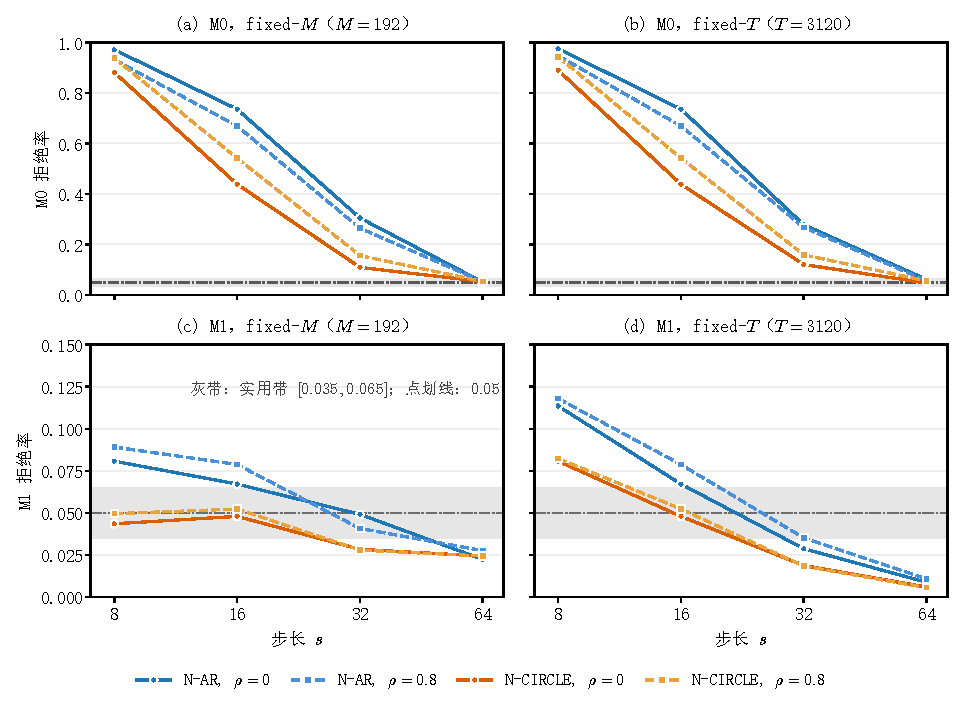
\includegraphics[width=0.96\textwidth]{../artifacts/figures/FigureB_BPI_H0_panels.pdf}
\caption{BPI 在两种预算制度与两种校准器下的零假设拒绝率（每格 $n=2500$）。(a)(b) 为 M0，纵轴 $[0,1]$；(c)(d) 为 M1，纵轴 $[0,0.15]$，两行量尺不同，曲线高度不可直接比较。灰带为实用等价带 $[0.035,0.065]$，点划线为名义水平 $0.05$；逐格分类仍依 Wilson 区间判据（\S\ref{sec:criteria}）。横轴为步长 $s$（对数刻度），连线只引导相邻设计点。实线/圆圈为 $\rho=0$，虚线/方块为 $\rho=0.8$；曲线未作平滑。}\label{fig:bpi-h0}
\end{figure}

\subsection{逐格校准分类}\label{sec:h0-classify}
112 个评价单元的四类计数见表~\ref{tab:calibration}。M0 在两种表示下均有 $20/28$ 个配置被判为实质反保守、没有配置被判为实质保守；M1 的分类分散于四类，说明依赖感知乘子改变了校准图谱的形态，却未实现统一校准。这些计数描述预设网格内的有限样本分布，不是方法在更广参数空间中的“通过率”。以固定窗口数、N-AR、$\rho=0$、BPI 为例，M0 在 $s=8,16,32$ 均为实质反保守、$s=64$ 转为实用校准；M1 随步长增加依次经历实质反保守、未定、实用校准与实质保守。这里报告的只是相邻格点的观测状态变化，不估计两点之间的连续临界步长（完整清单见补充材料 S1）。

\begin{table}[t]
\centering
\small
\caption{两种表示与两种校准方法的逐配置校准分类}\label{tab:calibration}
\begin{tabular}{llcccc}
\toprule
表示 & 方法 & 实用校准 & 实质保守 & 实质反保守 & 未定\\
\midrule
BPI & M0 & 7 (25.0) & 0 (0.0) & 20 (71.4) & 1 (3.6)\\
BPI & M1 & 5 (17.9) & 10 (35.7) & 7 (25.0) & 6 (21.4)\\
MOMENTS & M0 & 6 (21.4) & 0 (0.0) & 20 (71.4) & 2 (7.1)\\
MOMENTS & M1 & 1 (3.6) & 12 (42.9) & 7 (25.0) & 8 (28.6)\\
\bottomrule
\end{tabular}

\vspace{0.2em}
\begin{minipage}{0.95\textwidth}
\footnotesize 注：每行包含 28 个配置；括号内为百分比。分类判据见第~\ref{sec:criteria}~节。
\end{minipage}
\end{table}


\subsection{预设主对比}\label{sec:h0-primary}
表~\ref{tab:primary}报告 P1--P3 的点估计、边际 $95\%$ basic 自助区间与 Holm 校正结果。P1 与 P2 分别为 $0.5354$ 和 $0.5330$，区间下界均远高于预设阈值 $0.10$；P3 为 $0.0266$，区间整体高于 $0.01$，三项经 Holm 校正后 $p$ 均为 $0.00030$。因此，在两个预设数据生成过程、$\rho=0$ 与 BPI 表示的等权平均意义下，重叠端相对非重叠端的 M0 失校准超过 10 个百分点，且非重叠端的 M1 存在可检测的保守偏差；该结论不延伸为每一数据生成过程、依赖水平或表示下的必然规律。

对次级描述而言，原序列依赖对步长对比的修饰方向随生成过程与表示而异：$\rho$ 由 $0$ 变为 $0.8$ 时，$s=16$ 相对 $s=64$ 的拒绝率差异变化量介于 $-0.1148$ 与 $0.1032$ 之间，符号并不一致（定义与完整八值见 S7），故不提出依赖具有统一单调作用的结论。

\begin{table}[t]
\centering
\small
\caption{预设主对比 P1--P3 的效应估计与推断结果}\label{tab:primary}
\begin{tabular}{llccc}
\toprule
对比 & 估计量 & 点估计 & $95\%$ basic CI & Holm $p$\\
\midrule
P1 & fixed-$M$：$s{=}16$ 减 $s{=}64$（M0） & 0.5354 & $[0.5210,0.5494]$ & 0.00030\\
P2 & fixed-$T$：$s{=}16$ 减 $s{=}64$（M0） & 0.5330 & $[0.5194,0.5462]$ & 0.00030\\
P3 & $0.05$ 减 M1（$s{=}W{=}64$，fixed-$M$） & 0.0266 & $[0.0224,0.0308]$ & 0.00030\\
\bottomrule
\end{tabular}

\vspace{0.2em}
\begin{minipage}{0.95\textwidth}
\footnotesize 注：均针对 BPI 与 $\rho=0$，并对两个生成过程等权平均；区间为边际 $95\%$ 基本型自助置信区间，$p$ 为 Holm 调整后的单侧值。对比与阈值定义见第~\ref{sec:criteria}~节。
\end{minipage}
\end{table}

